 \documentclass{standalone}
% preamble: usepackage, etc.
\begin{document}

\chapter{图同构的数学推理引擎的设计和构建}
\section{系统概述}
在研究设计图匹配推理引擎之前,先介绍一下<<初等数学问题求解关键技术
及系统>>课题。该系统的研究内容主要包括初等数学问题的题意理解和初等
数学问题自动求解两大部分。题意理解就是面向初等数学领域的自然语言处理,
会根据数学领域的自然语言特性,研究针对数学领域的中文分词、词性标注、
命名实体识别、关系抽取、句法分析等自然语言处理基础技术。另一部分,
主要就是根据初等数学问题自然语言理解之后的语义表示,结合问题归约、
认知模型、自动推理、大数据深度学习、图嵌入、符号计算等技术,自动
求解问题并重构类人解答过程。从上述的介绍中可以看出,图匹配推理引擎
主要完成整个系统的第二部分工作,是自动推理的核心部分。本文最终设计了计算推理与逻辑推理是交互式的推理思想,两种
推理方式相辅相成,让整个推理引擎的功能更加强大,解题的覆盖面也更加广泛。
本章后续的具体小节,将会对图匹配推理引擎与符号计算推理做出详细深入的研究
阐述。类人解答系统的结构和流程如图4-1所示。

\begin{figure}[htbp]
	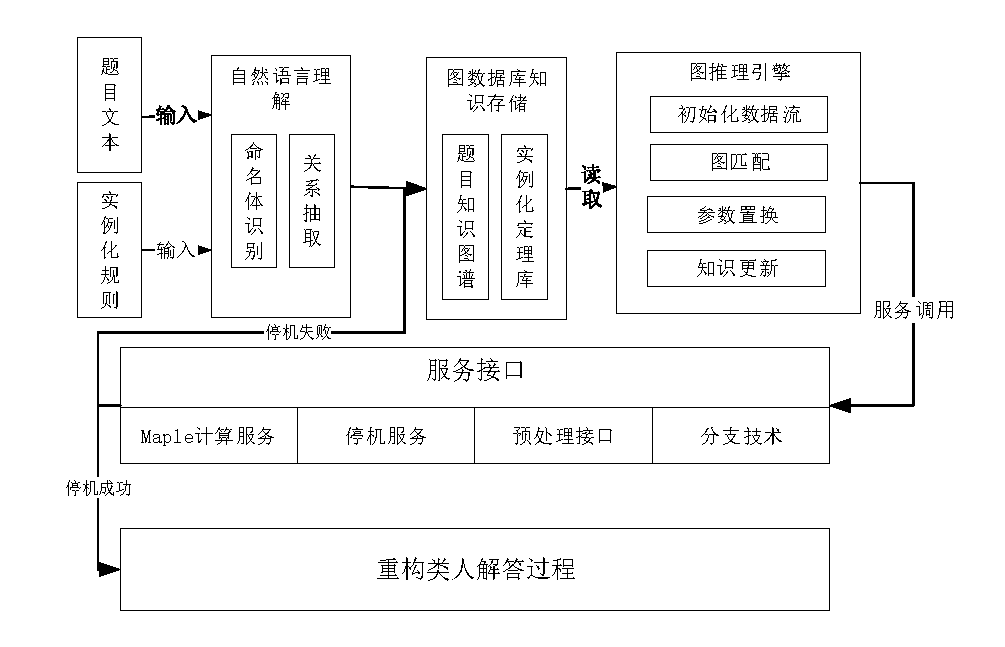
\includegraphics{系统架构图.pdf}
	\caption{基于初等数学的类人解答系统}
	\label{系统架构图}
\end{figure}
从系统架构图中可以看出,类人解答系统共分为5个部分:系统的输入和输出、
知识理解、知识存储、以及自动推理。系统输入包括两部分,第一部分是待
求解的题目文本,这里的文本是需要处理文本中公式和符号,系统接受的文本
输入是经过latex处理过的文本。同样的,对于实例化规则的文本描述也需要
将其中的公式转成latex格式。知识理解主要是指利用自然语言理解的相关技术
去生成机器可以理解的形式,自然语言理解通过命名体识别和关系抽取的技术手段
生成<实体-关系-实体>三元组的来表示每一句描述的语义。而一段文本则用三元组
数组的形式去存储,最终为了前后端交互方便,自然语言的结果以json的数据格式
进行保存和跨平台传输。后端接受到前端自然语言理解的json数据后,进入知识
存储和表示模块。为了发挥图的优势,选择使用知识图谱来表征知识,存储在图数据
库中。无论是题目json文件还是实例化规则的json文件都以知识图谱来存储知识,
然后存储在neo4j图数据库中,不同的是实例化规则是提前批量将json文件生成
存储在图数据库中,形成实例化规则库,而题目是动态的生成知识图谱并存储,在
正确求解完之后将原题目的图谱删除掉。

自动推理和求解主要是依赖于推理引擎去实现。本文设计和构建的推理引擎是
基于图同构的匹配置换算法的实现,并融合了计算和逻辑双重交互推理方式。
整个推理引擎的设计使用分层结构,共分为四层逻辑结构,每一层相互独立,
又层层递进并存在一定的调用和依赖关系。第一层,是读取题目图谱和实例化
图谱,对图谱进行解构成内存中最小的推理形式-三元组,因此用三元组集合
逻辑上来表示图。在解构的同时会完成内存中各种推理数据结构的初始化工作。
第二层,是对题目图谱和实例化规则图谱进行匹配,匹配的结果分为两种:
匹配成功和匹配失败。匹配成功会进入到下一层逻辑,匹配失败会停止当前
实例化规则的推理,继续去实例化库中选取新的实例化定理。第三层,参数置换
层是完成实例化形式参数到题目具体参数的映射。第四层,知识更新层是对
第三层生成的新知识进行知识的插入更新。计算推理主要是在推理引擎的
第三层逻辑中提供相对应的计算服务,计算服务则是依赖于符号计算平台
Maple作为基础支撑。

\section{复杂逻辑推理研究}
所谓复杂逻辑推理,顾名思义,即多种推理方式、策略的有机结合而形成的一种
复合的推理方式。相对于单一的推理方式,复合的推理方式不仅能更加准确、
全面的模拟人类的逻辑推理思维过程,还能极大提高系统的解题能力和稳定性。
除此之外,更多的推理方式融合会很大程度上提高了系统的容错率和兼容性。
传统的复杂逻辑推力组合包括基于规则的正向推理与基于规约的逆向推理,
经典分析法与反证法融合推理等。
\subsection{正向推理}
正向推理是从已知事实出发,通过规则驱动,不断产生新的知识实体的一种
推理方式。基于实例化规则的正向推理基本思想是已知事实在规则的驱动下
产生新知识实体,然后新的知识插入到原始事实中去,继续规则驱动,这样
不断知识迭代的一个过程。知识迭代的终止条件就是产生的知识与求解目标
相匹配,表示到达求解目标,求解成功,终止正向推理。如果新产生的知识
与目标知识不匹配,则会将新知识插入到原有的知识库中继续实例化规则匹配,
直到所有实例化规则均不能匹配出发产生新的知识为止。此时表示正向推理
失败,结束正向推理。正向推理的详细推理过程如下图4-2所示:

\begin{figure}[htbp]
	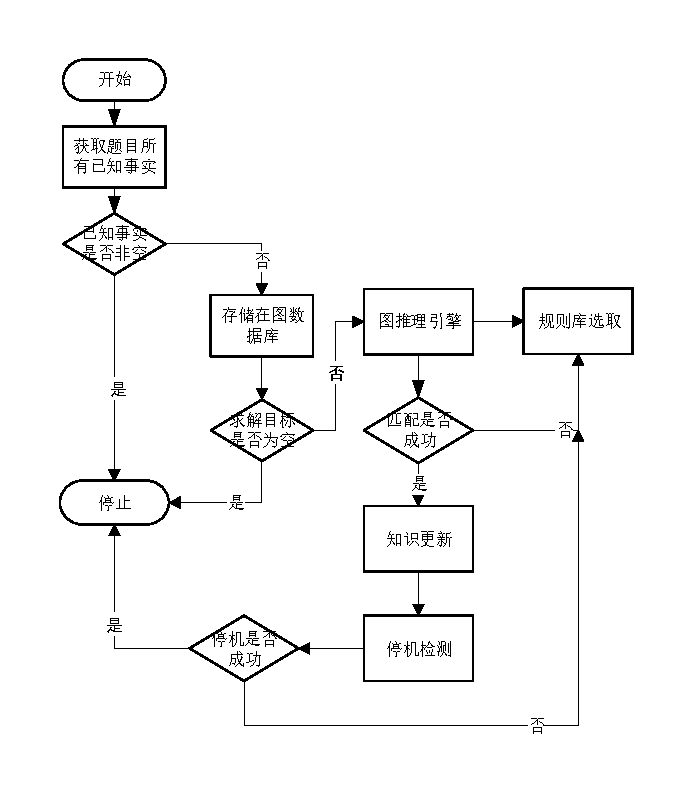
\includegraphics{正向推理1.pdf}
	\caption{正向推理流程图}
	\label{正向推理1}
\end{figure}
由正向推理的流程可以得出,推理的终止条件是在已知事实和求解目标
非空的前提下,停机服务会对每次实例化规则产生的新知识与求解目标
比对,若求解目标与新知识一致,这里的一致同样是定义的三元组等价。
正确停机是正向推理以及逆向推理的关键,为了保证系统运行的稳定性,
不延迟、不错误、不超时是对停机服务基本的要求。

\subsection{逆向推理}
逆向推理是从目标结论出发,采用分解子目标和规约的基本思想,通过对目标
结论的等价变换、分解成多个子目标的形式,然后从子目标出发,利用分支的
技术,并行规约不同的子目标,一步步递归逆向直到搜寻到已知事实。
其算法描述如下:
\begin{algorithm}[H]
	\KwData{A set of questionTriplesSet}
	\KwResult{The tree of rule's node}
    Begin reverse reasoning\;
	\If{questionTriplesSet == null || all facts is satisfied} {
		return;
    }
	\If{questionTriplesSet != null} {
		Search conclusion triples in the questionTriplesSet\;
		\quad Divide the conclusion triples into multiple sub-conclusion\;
    }
	New Branch reasoning\;
	\If{sub-conclusion triple is contained in the map of triple to rule} {
    	Get the rule from the map\;
		\quad Get the condition triple from the rule\;
		 \If{If questionTriplesSet contain condition triple} {
    		\For{all triple in rule condition triples}{
   	  			dfs(triple)\;
   }  
    	}
    }
	\caption{逆向推理算法}
	\label{dfs}
\end{algorithm}
\subsection{正逆结合}
正逆结合是一种融合了正向推理和逆向推理的复杂逻辑推理方式,这种混合的
推理方式具有兼容性强、推理效率搞、推理方式多样,能较好的模拟人类解题
思维过程等优势。与单一的推理模式不同的是,正逆结合的推理方式,可以
综合已知事实和目标结论,参与推理的信息更加丰富,同时在推理的过程中
两种推理方式也起到互补作用,给各取所长。正逆结合推理分成”先正后逆“、
”先逆后正“两种不同方式。本文最终选择了”先逆后正“的方式进行推理。首先,
逆向推理是系统的入口,逆向推理的主要功能是提高实例化规则选取的效率,
解决正向暴力匹配实例化规则的时间复杂度过高问题。逆推就是通过分解子目标
以及等价规约求解目标,然后递归的去搜寻实例化知识库,递归的终止条件是
已经搜寻到已知事实,并由此构建一棵推理规则树。然后通过逆向推理构建的
规则树回溯出解题路径,将解题路径对应的实例化规则作为正向推理的输入,
开始正向匹配,产生新知识。为了进一步提高解题的效率,正推和逆推中都
使用了分支并行推理技术。

一般而言,双向推理融合正向推理与逆向推理有三种组合方式:”先正后逆“、
”先逆后正“、”正逆同时“。本文采用是”先逆后正“的推理方式,以下小节将
详细介绍”先逆后正"的双向推理流程和算法。

\subsection{先逆后正}
采用“先逆后正”组织结构的双向推理,是将逆向推理作为正向推理的一个重要
补充,逆向推理是构建解题路径的规则树,然后再通过回溯算法输出解题的实
例化规则路径,路径中的每个节点对应就是正向推理的实例化规则,这个路径
作为正向匹配的输入,从而产生每个路径节点对应的新知识。逆向推理相当于
根据已知目标结论出发,有目的性的搜索解题中所使用的实例化规则,这样很
大程度上提高了正向暴力式匹配所带来的时间开销。

“先逆后正”双向推理算法中,逆向推理最基本的思想是分解子目标和等价归约,
然后不断递归这个过程,最终生成包含解题路径的规则树,对于规则树进行回溯
生成解题路径,解题路径则作为正向推理的输入。如下图4-3是本文的“先逆后正”
推理算法思想的框架图。

\begin{figure}[htbp]
	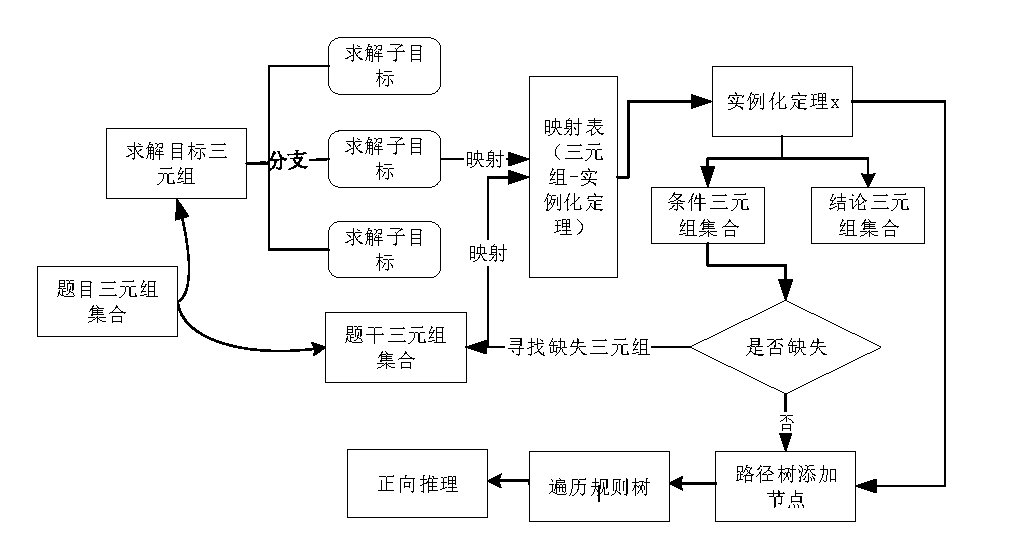
\includegraphics{正逆结合推理.pdf}
	\caption{“先逆后正“推理框架图}
	\label{正逆结合推理}
\end{figure}

\section{图匹配推理引擎的构建与设计}
图匹配是个经典的图上匹配问题,图匹配问题涉及二分图匹配、最大连通域匹配、
子图匹配等问题。本文设计的图匹配引擎采用的算法思想就是子图匹配算法,又
称子图同构算法。所谓子图同构任务,即给定一个target graph A(m,n),和
一个query graph B(p,q)。其中,m、p是点集,n、q是边集。试图寻找一种
映射关系,使得两个图对应的点label相同,query graph中的边在target 
graph中对应的点之间都存在,且label相同。如下图3-4所示:
*****************
左边图可以同构到右边的上面三角,或者下面三角。
\subsection{引擎基本设计思想}
图匹配推理引擎核心思想是基于图同构的搜索匹配,并寻找一组置换等价的
映射集的复杂逻辑推理引擎。上文已经对图同构进行了阐述,图匹配推理引擎
由图同构的判断器、置换合一的生成器以及知识冲突消解的处理器三大部分
组成。同时也融合了符号计算平台的计算服务、停机等外部接口,为推理引擎
提供计算和停机服务。另外,引擎中还引用了分支并行技术,很好的解决了
多解、分类讨论、等价变幻、知识分解等一些列较为复杂问题,也提升了引擎
并行处理的能力和解题速度。下图4-5是推理引擎的详细结构设计图。

\begin{figure}[htbp]
	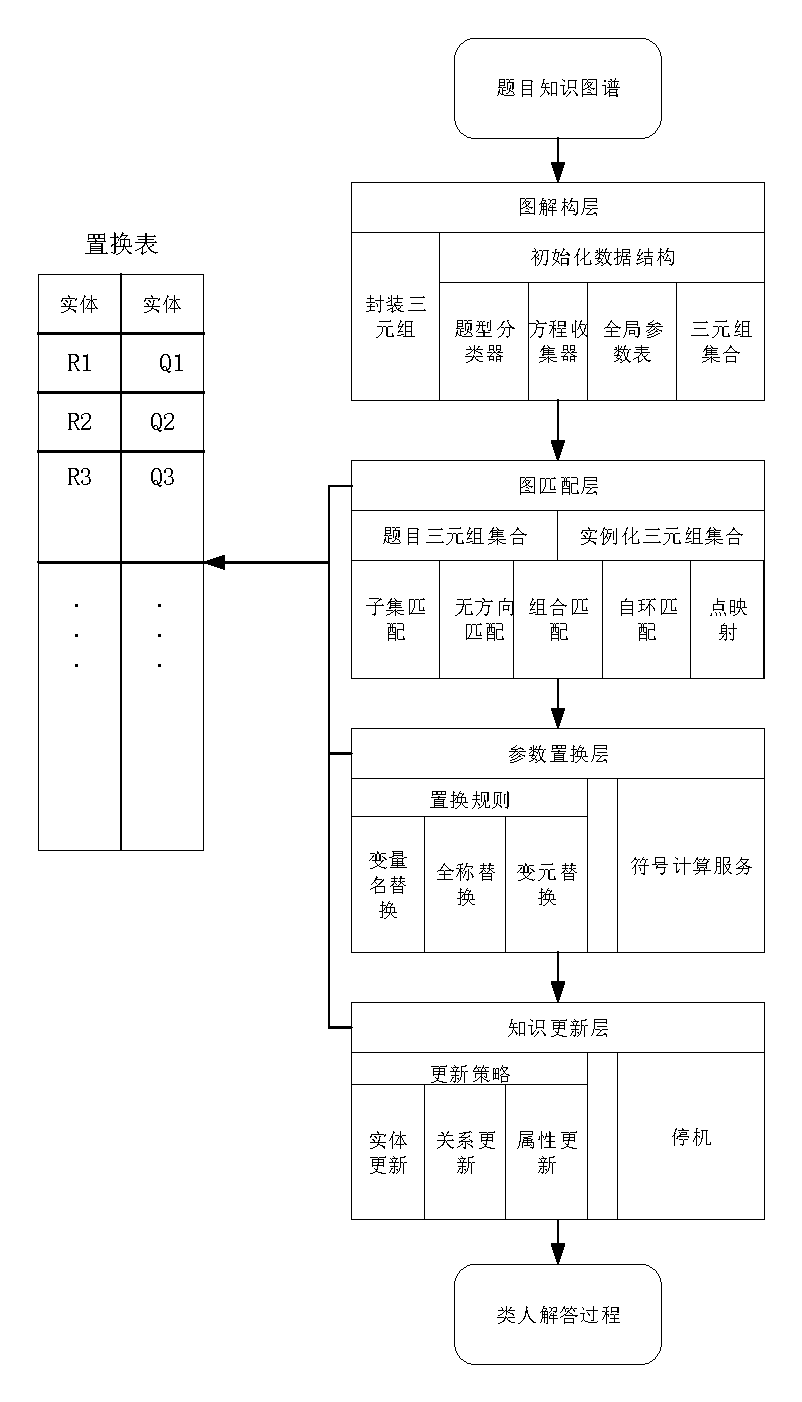
\includegraphics{推理引擎.pdf}
	\caption{推理引擎逻辑架构图}
	\label{推理引擎}
\end{figure}
从图中可以看出,************

\subsection{逻辑架构}
图匹配推理引擎共分为四层逻辑结构,每层结构保持相对独立性。第一层逻辑
结构,图解构层。该层是整个推理的入口,子图的读取就是引擎的输入,对输
入的子图进行解构并转换成推理的数据结构,同时初始化内存各种推理数据流。
下图3-6是推理引擎的第一层逻辑结构图。
*****************
从图中可以看出,*************
第二层逻辑结构,图匹配层。该层是引擎核心部分,具有图同构的判断器和
置换映射集的生成器。第三层逻辑结构,变量置换层。该层依赖于图匹配层,
变量置换的是依据置换映射集生成器生成的置换表,找出若干组变量置换。
同时,该层还调用符号计算平台服务,置换出的变量映射是符号计算接口的
输入参数。第四层逻辑结构,知识更新层。该层是对于变量置换层生成的
新知识进行处理,主要包括知识插入和知识冲突消解两种方式。知识插入
是完成下一轮匹配搜索迭代的前提,知识冲突消解是包括两个部分,知识异常
检测以及知识的冲突检测处理。其中知识异常是指新生成的新知识出现空指针
、不合法、矛盾等情况;知识冲突检测是指新生成知识与已有的知识产生冲突,
需要相应的策略和规则去处理新旧知识,防止出现知识丢失、冗余、重复。

\subsection{Match Engine}
从上文的阐述中,可以看出匹配是整个引擎设计的核心部分。本节会更加详细的
阐述逻辑结构的第二层,图匹配层的整个设计思想和具体结构。下图4-7是图匹配
详细结构图。

\begin{figure}[htbp]
	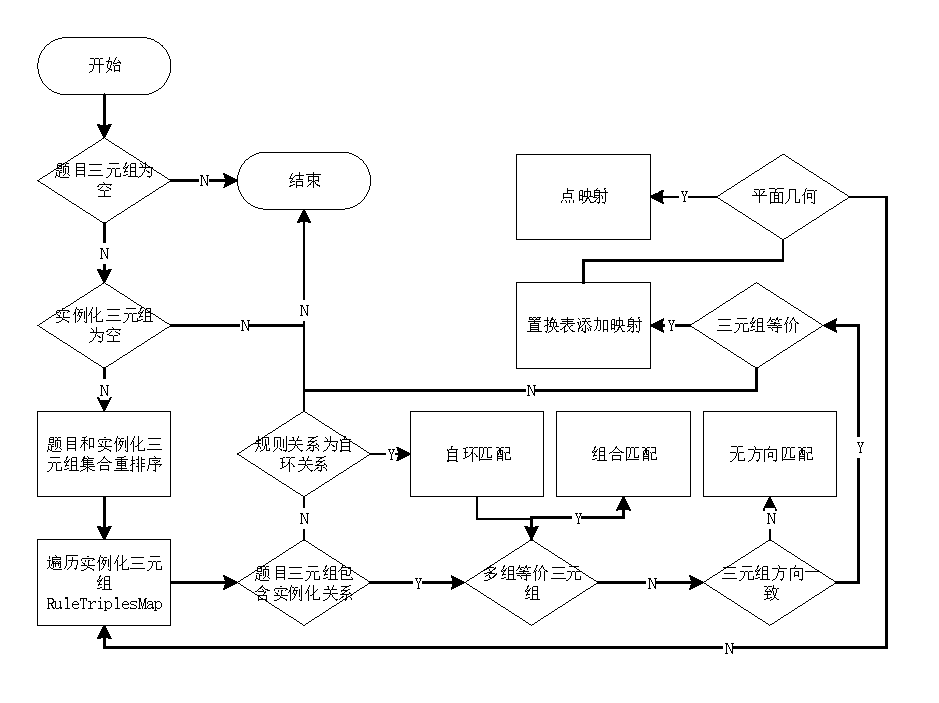
\includegraphics{图匹配算法1.pdf}
	\caption{图匹配算法流程图}
	\label{图匹配算法1}
\end{figure}
从图中可以看出,***********

\subsection{匹配原则}
本引擎匹配最核心的思想,是寻找两组三元组集合是否满足最小子集思想。通过
上文的介绍,题目子图和实例化规则子图都会解构成三元组集合,重新定义三元组
equal的标准:实体类型相同,关系名相同。引擎将实例化规则三元组集合作为最
小子集,在题目三元组集合中搜寻是否覆盖最小子集,为了保证匹配准确度,需要
遵循子集匹配、无方向匹配、组合匹配、自环匹配、点映射这五条基本准则。下面将分小节
详细介绍每种匹配原则。其伪代码描述为:
\begin{algorithm}[H]
	\KwData{question graph and rule graph}
	\KwResult{datastream of matching}
    Begin match reasoning\;
	\quad divide question graph and rule graph into 
	\\questionTriplesList and ruleTriplesList\;
	\If{questionTriplesList == null || ruleTriplesList == null} {
		return;
    }
	Resort questionTriplesList to qMap and Resort ruleTriplesList to rMap\;
	\For{all question relation(qr)  in rMap's keySet}{
		\For{all rule relation(rr) in qMap's keySet}{
			\If{qMap contains qr} {
		Select five matching strateges\;
		\If{rTriple match to multi-qTriples} {
		Enter into conbinationMatch model\;
		\If{Exit the fake match conbination} {
		delete the fake match conbination\;
    }
		Refresh the Map of questionEntity to ruleEntity\; 
		 
    }

    }
  		 	}  
   		}
		\eIf{matching is not successfully} {
			Print some error log about match\;
			return;
    }{
		enter into next model,continue reasoning\;
	}  
	
	\caption{匹配算法}
	\label{dfs}
\end{algorithm}
\subsubsection{子集匹配}
子集匹配是保证引擎有较好兼容性和通用性的一个重要原则。子集匹配的对象是
三元组中实体类型。子集匹配的定义:给出两组三元组,若它们的实体类型具有
继承关系,可以是直接的父类子类继承,或满足间接继承关系,则两组三元组满足
子集匹配。下面以一个例子进行说明,题目三元组<等差数列-项关系-首项>,规则
三元组<数列-项关系-项>,等差数列直接继承于数列,首项直接继承于项,因此
两个三元组满足子集匹配原则,属于可匹配三元组。
\subsubsection{无方向匹配}
无方向匹配是增加引擎匹配搜索灵活性,增大了匹配搜索的范围。知识图谱中
存储的题目和实例化规则子图都是以有向图形式存储的,因此三元组均是有方
向的。无方向匹配原则是指将三元组匹配进行两次匹配检测,第一次完成正向
就检测,匹配成功退出返回0;匹配失败则将三元组进行逆向匹配检测一次,
匹配成功退出返回0,匹配失败返回-1。例如,题目三元组<反比例函数-区间关系-区间>,
实例化三元组<区间-区间关系-反比例函数>,则需要进行两次匹配检测,满足
无方向匹配原则,属于可匹配三元组。
\subsubsection{组合匹配}
组合匹配是指一个三元组或一组三元组能匹配上两组或两组以上的三元组集合,
这个时候边会出现组合问题。组合匹配形式主要有一对多,多对多的情形。从
形式定义和概念上组合匹配较为容易理解,但是如何正确的处理组合分支、
组合爆炸是个比较疑难的问题。本文对于组合匹配问题采用了多重解决方案,
并在具体题目得以验证和应用。当遇到组合匹配时,基本原则是将组合匹配
转换成单一匹配,然后通过循环的方式去完成组合。组合的情况较为复杂,以下
将通过例子来列举组合发生的几种情况。

例1,实例化三元组<数列-项关系-项>,题目三元组集合{<等差数列-项关系-首项>,
<等比数列-项关系-项>},这是最常见的三元组组合情形,引擎处理的手段是将题目
三元组集合拆成等价于最小实例化三元组的多组,然后依次匹配或采用分支技术并
行匹配。例2,实例化三元组{并集AuB-子表达式关系-集合A,并集AuB-子表达式关系-集合B}
题目三元组{并集MuN-子表达式关系-集合M,并集MuN-子表达式关系-集合N,
并集PuQ-子表达式关系-集合P,并集PuQ-子表达式关系-集合Q},此组合
对应于多对多的一种情形,若按照组合学方案会有6种组合方式,这样会产生
4组多余的组合出来,若四组知识继续插入到知识库,进行下一轮的匹配循环
迭代会继续产生越来越多的知识,最终便会组合爆炸。如何寻找有效组合,排除
假组合,将在下文详细介绍。

对于上文例2的组合情形,引擎会启用三种机制去筛选假组合。方案一:属性标价法。
属性标记法,是通过在关系中添加一个属性字段isGroup来标记三元组是否属性同一组,
同一组的定义是两个或两个以上三元组具有共同的头实体或尾实体。属性标记法通过
属性字段来对相同三元组进行分类处理,先分类再匹配,这种方式可以有效的降低
组合次数,例2中题目三元组四个相同三元组,通过isGroup属性标记分类,化分成
{并集MuN-子表达式关系-集合M,并集MuN-子表达式关系-集合N}和
{并集PuQ-子表达式关系-集合P,并集PuQ-子表达式关系-集合Q}两类,分类完成后将
原有的随机组合6组降成为2组有效组合,筛选掉4组多余组合,大大提升了匹配效率。
\subsubsection{自环匹配}
自环匹配是弥补匹配设计缺陷,匹配的最小单位是三元组,因此匹配子图的限制条件
确保能解构成三元组集合,不能存在离散的孤立节点。为了让推理引擎通用性更高,
引擎对孤立节点情况做了自我完善。当实例化规则子图中出现自环节点时,引擎
会自动检测同类型的题目节点并增加一条自环关系,解构后的三元组集合多出相应
的自环三元组。
\subsubsection{点映射}
点映射是匹配策略中比较特殊的一种情形,应用场景主要是针对平面几何和解析几何
中。在平面几何和解析几何中常常会出现多边形、线段、角、边、点这些描述,且
多边形、线段、边、角都包含点的信息,若采用预处理方案将所有的点的信息全部
扩展出来,点与边、点与多边形、点与线段之间会有着复杂的关系描述,进行知识
表示时会形成较为复杂的图谱,进而会导致匹配时组合爆炸以及后续知识爆炸问题。
为了解决平面几何中这一问题,引入点映射简化知识表示。点映射思想是在知识表示
环节省去隐含点的信息,简化图匹配的复杂度,生成置换表结构后,再进行点的
轮换映射处理,即将图中点的知识扩展问题转化成匹配后的置换表中的点的映射
轮换问题。例如图3-1所示,图中左边部分是题目图谱,右边是”等腰三角形两腰相等“的实例化图谱。

********************
如表3-1(a),3-1(b)分别是点映射前的置换表和点映射后的轮换表。
\begin{table}[h]
	\caption{点映射前置换表} 
	\begin{tabular}{|c|c|} 
		\hline  
		实例化实体 & 题目实体\\
		\hline  
		A'B'C' & ABC  \\  
		\hline 
		A'B' & AC  \\  
		\hline 
		A'C' & BC\\  
		\hline  
	\end{tabular}
	\label{tablea}
\end{table}

\begin{table}[h]
	\caption{点映射后置换表} 
	\begin{tabular}{|c|c|c|c|} 
		\hline  
		实例化实体 & 第一次轮换 & 第二次轮换 & 第三次轮换\\
		\hline  
		A'B'C' & ABC  & ABC & ABC\\  
		\hline 
		A'B' & AC  & AC & AC\\  
		\hline 
		A'C' & BC & BC & BC\\    
		\hline  
		A' & A & B & C\\  
		\hline 
		B' & B & C & A\\  
		\hline 
		C' & C & A & B\\  
		\hline  
	\end{tabular}
	\label{tablea}
\end{table}
\subsection{置换等价}
置换等价是推理引擎中另一核心问题,处于推理引擎的第三层逻辑结构,它是匹配层
和知识更新层的桥梁,起到知识传递作用,同时置换等价的结果作为符号计算服务
的参数输入,直接关联到知识产生的正确性。本文结合数学知识图谱的具体特点,
在推理引擎中使用的是广义上的置换,为了求解实际复杂的问题,实现形式化
参数到实际参数的替换,置换的类型更加多样。

图匹配推理引擎中共使用了五种置换手段:实体置换、分类置换、全称置换、
变量名置换、参数置换。实体置换指的是知识图谱上实体和关系的置换,依赖于匹配算法,
对于题目图谱和实例化规则图谱匹配生成的实体置换表,这是引擎置换的第一步。
分类置换的定义较为简单,是指引擎为了处理不同类型的数据采用不同的置换策略,
例如,函数的自变量置换和数列的角标置换是不同类型,需要分类处理,分类置换在
引擎中使用广泛。全称置换、变量名置换、参数置换可以统称为字符串匹配中的符号置换,
具体三种置换方式的详细解释在第三章的小节中进行了详细介绍和举例说明,三种置换
可以看作是字符串符号置换的粒度不一样,其中全称置换的粒度最粗,参数置换的粒度最细。
选取哪种字符串的符号置换,同样需要依据具体题目输入的数据和实例化中待置换的数据。
如下表是实例化实体二次函数$f(x)=a*x^{2}+b*x+c$和题目实体二次函数$g(x)=x^{2}-3$的四种置换策略。
\begin{table}[h]
	\caption{置换等价策略} 
	\begin{tabular}{|c|c|c|} 
		\hline  
		置换类型 & 置换前 & 置换后 \\
		\hline 
		实体置换 & \makecell[l]{实体\{name:$f(x)=a*x^{2}+b*x+c$,
		\\type:二次函数\}}   
		& \makecell[l]{实体\{name:$g(x)=x^{2}-3$,
		\\type:二次函数\}}\\
		\hline  
		全称置换 & $f(x)=a*x^{2}+b*x+c$ & $g(x)=x^{2}-3$ \\  
		\hline 
		变量名置换 & $f(x)=a*x^{2}+b*x+c$ & $f(x)=x^{2}-3$ \\  
		\hline 
		参数置换 & $f(x)=a*x^{2}+b*x+c$ & \makecell[l]{\{$a=1$,
		\\$b=2$,
		\\$c=-3$\}}\\  
		\hline  
	\end{tabular}
	\label{tablea}
\end{table}
\section{知识更新}
知识更新是当前轮匹配和下一轮匹配迭代的重要衔接。引擎处理知识更新的技术手段,
知识插入、冲突消解、更新回代、自动停机等。知识插入是对实例化规则产生的新知识
插入到原有的题目知识图谱中,是知识更新最基础也是最重要的手段。知识更新流程如
下图4-8所示:

\begin{figure}[htbp]
	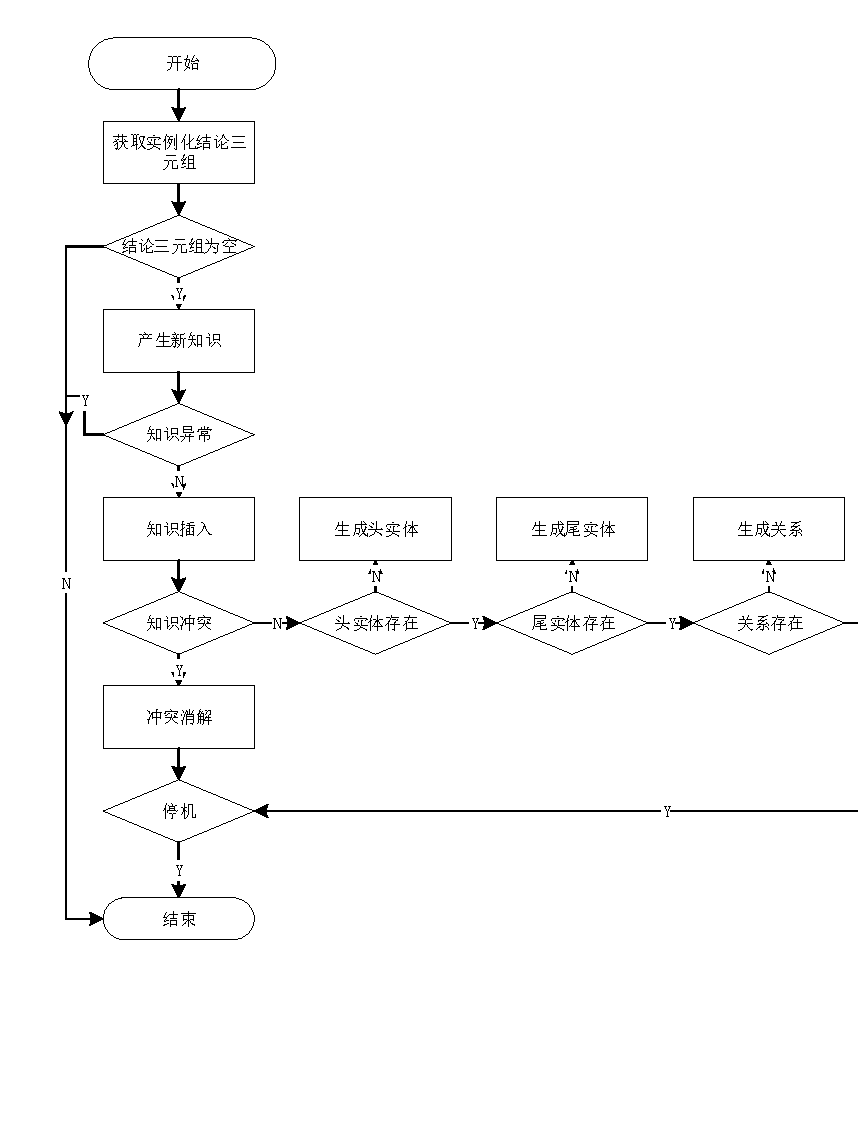
\includegraphics{知识更新1.pdf}
	\caption{知识更新流程图}
	\label{知识更新1}
\end{figure}
根据图4-8所示的知识更新流程图的描述,其对应的知识更新算法伪代码解释如下所示:
\begin{algorithm}[H]
	\KwData{A group of new knowledges}
	\KwResult{Insert knowledges into question graph correctly}
    Knowledge exception detach\;
	\If{Knowledge is null or illegal} {
		end refresh\;
		return;
    }
	\If{match successfully} {
		Get conclusion triple\;
		\quad Calculator Integer variety the refreshTag of refresh type\;
		\If{refreshTag > 0 \&\& refreshTag <= 3} {
		select the refresh strateges according to the refreshTag\;
		\If{new knowledge is confilct with exit knowledges} {
		solve the confilct betwwen new knowledge and exit knowledges\;
		\If{stop conditions are satisfied} {
		end reasoning\;
		return;
    }
	
    }
    }
    }
	\If{Knowledge type belong to Equation type} {
		Add the Knowledge into Equation Collector\;
		return;
    }
	
	\caption{知识更新算法}
	\label{dfs}
\end{algorithm}
从上述算法中,知识更新的依据来源于两部分:第一部分是引擎逻辑层的第三层符号计算
平台产生的新知识;第二部分是具体的知识插入策略,在知识更新之前,会将新知识封装
成三元组结构,再去解析实例化定理中的结论三元组,结论三元组有5种不同情形,每种
情形对应一种更新策略,具体更新策略如表4-1所示。
*********************

知识更新是正向推理迭代思想至关重要的环节,算法中冲突消解体现在知识合法性检测上。
冲突消解有以下几种情景:

1)新知识为空或者空字符串

2)出现恒等式、矛盾式,如“1=1”,“1=-1”

3)多解,知识冗余

4)新知识插入时已经存在同类型的知识,类型变元相同或者重复都会造成冲突。

\section{类人解答过程的构建}
类人解答过程的构建是类人自动求解系统的输出部分,它是将系统从自然语言理解部分
到预处理的变量引入,然后到后端的推理引擎规则推理和计算推理,形成类似人答题的
逻辑思维,最终用“因为...,所以...."因果逻辑来展示整个推理过程。此模块是依赖于推理模块的逻辑推理和计算推理,在推理的同时构建解答
过程规则树,规则树的节点代表使用的规则或者定理,最终的输出就是对规则树进行回溯,得到类人解答过程,适用范围
是选择题、填空题、非图表类解答题。输出的形式是两种,第一种是后端以Log日志的方式;
方式二是知识图谱的形式呈现解答过程子图。

\subsection{构建规则树}
规则树是用树状结构去保存推理过程中产生的路径。树中的节点对应求解中应用的知识,
知识来源有原始题目信息生成的节点,推理中使用的实例化定理生成的节点,
计算推理产生的方程知识节点,以及表达式的统一化简产生的知识节点。首先,定义
树中节点的类结构,**********************。具体规则树构建算法流程如下:

1)将题目中的所有原始节点作为树的第一层节点

2)进入推理模块,若产生新知识,执行算法步骤3);否则继续推理

3)新知识是否触发分支,若触发分支,开启分支推理;否则执行
算法步骤4)

4)将新知识节点添加到树中,并关联其所有父节点,重复
执行算法2-5),直至停机

\subsection{重构类人解答}
重构类人解答过程一般分为两步:一,在推理过程构建解答过程规则树,
并对树中每个节点编号;二,对规则树进行回溯算法,生成可读过程和
解答过程子图。节点编号得满足两条约束:1)同一层节点之间的编号按照
从左至右的顺序依次编号;2)父节点的编号理应小于子节点编号。编号是在
构建节点的同时完成,并作为节点的属性字段存储,方便回溯遍历时输出相对应的
编号。类人过程时通过回溯算法去找出树的路径,先深度优先搜索找出对应的因果
逻辑关系,然后再回溯找出所有的因果逻辑。若出现一题多解的情形时,利用分支
+回溯的算法,可以得到多组类人解答过程。

\begin{table}[h]
	\caption{计算$2m\times 2m$理想导体平板时域感应电流采用的三种存储方式的存储量比较。} 
	\begin{tabular}{|c|c|c|c|} 
		\hline  
		时间步长 & 非压缩存储方式 & 完全压缩存储方式 & 基权函数压缩存储方式 \\
		\hline 
		0.4ns & 5.59 MB & 6.78 MB & 6.78 MB\\  
		\hline  
		0.5ns & 10.17 MB & 5.58 MB & 5.58 MB \\  
		\hline  
		0.6ns & 8.38MB & 4.98 MB & 4.98 MB \\  
		\hline  
	\end{tabular}
	\label{tablea}
\end{table}

如图\ref{picd}所示给出了时间步长选取为0.5ns 时采用三种不同存储方式计算的
平板中心处$x$方向的感应电流值与IDFT 方法计算结果的比较,……。如图\ref{pice}
所示给出了存储方式为基权函数压缩存储方式,时间步长分别取0.4ns、0.5ns、0.6ns
时平板中心处$x$方向的感应电流计算结果,从图中可以看出不同时间步长的计算结果基本相同。

由于时域混合场积分方程是时域电场积分方程与时域磁场积分方程的线性组合,因此时域混合场积分方程时间步进算法的阻抗矩阵特征与时域电场积分方程时间步进算法的阻抗矩阵特征相同。

\begin{figure}[h]
	\subfigure[]{
		\label{picd}
		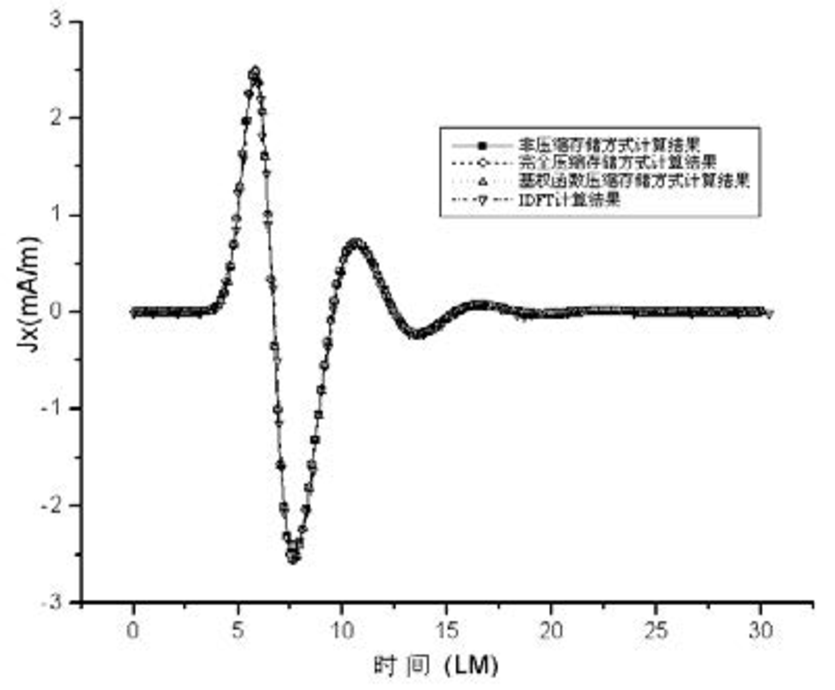
\includegraphics[width=6.77cm]{picd.pdf}}
	\subfigure[]{
		\label{pice}
		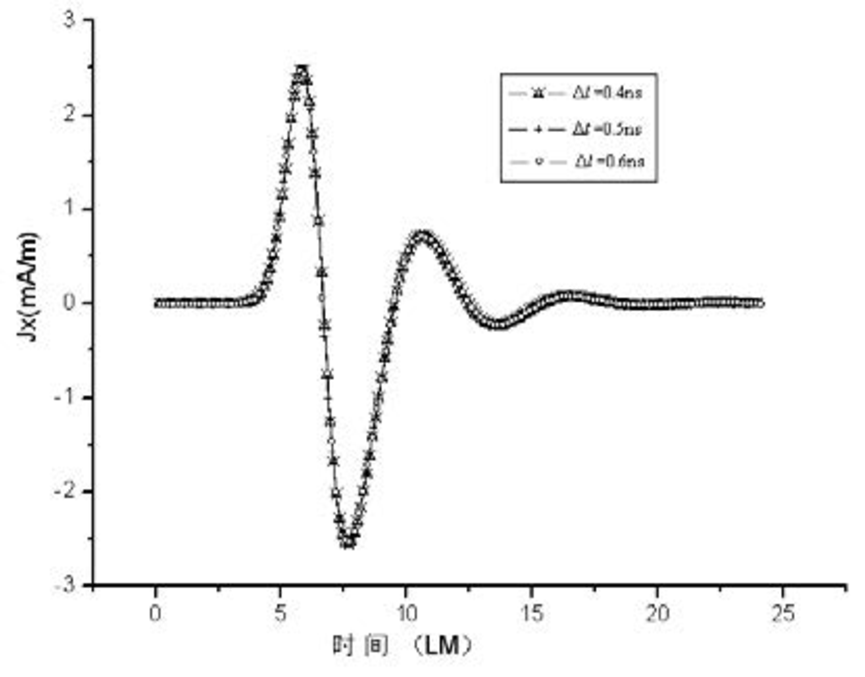
\includegraphics[width=7.04cm]{pice.pdf}}
	\caption{$2m\times 2m$的理想导体平板中心处感应电流$x$分量随时间的变化关系}
	\label{fig2}
\end{figure}


由于时域混合场积分方程是时域电场积分方程与时域磁场积分方程的线性组
合,因此时域混合场积分方程时间步进算法的阻抗矩阵特征与时域电场积分方程
时间步进算法的阻抗矩阵特征相同。
\section{时域积分方程时间步进算法矩阵方程的求解}

\begin{theorem}
	如果时域混合场积分方程是时域电场积分方程与时域磁场积分方程
	的线性组合。
\end{theorem}
\begin{proof}
	由于时域混合场积分方程是时域电场积分方程与时域磁场积分方程的线性组
	合,因此时域混合场积分方程时间步进算法的阻抗矩阵特征与时域电场积分方程
	时间步进算法的阻抗矩阵特征相同。
\end{proof}
\begin{corollary}
	时域积分方程方法的研究近几年发展迅速,在本文研究工作的基础上,仍有以下方向值得进一步研究。
\end{corollary}
\begin{lemma}
	因此时域混合场积分方程时间步进算法的阻抗矩阵特征与时域电场积分方程
	时间步进算法的阻抗矩阵特征相同。
\end{lemma}

\section{本章小结}
本章首先研究了时域积分方程时间步进算法的阻抗元素精确计算技术,分别
采用DUFFY 变换法与卷积积分精度计算法计算时域阻抗元素,通过算例验证了计
算方法的高精度。

\end{document}